\documentclass{beamer}

\usepackage[utf8]{inputenc}
\usepackage[english,russian]{babel}
\usepackage{cmap}
\hypersetup{unicode=true}
\usepackage{graphicx}
\graphicspath{{images/}{slides/images}}


\title{02. Text Preprocessing}
\subtitle{Computational Methods for Text Analysis}
\author{Пестова Алена}
\institute{НИУ ВШЭ Санкт-Петербург}

\newcommand{\tb}[1]{\colorbox{yellow}{#1}\space}
\newcommand{\Sp}[1]{\colorbox{green}{#1}\space}
\newcommand{\Sn}[1]{\colorbox{red}{#1}\space}

%\usetheme{lucid}
\begin{document}

    \begin{frame}
        \titlepage
    \end{frame}

    \begin{frame}{Tokenization: N-grams}
        N consecutive words.
        \begin{block}{Unigrams}
            \alert<2>{Восторг} \alert<3>{внезапный} \alert<4>{ум}
            \alert<5>{пленил} .
        \end{block}

  \begin{block}{Bigrams}
  \alert<2>{Восторг} \alert<2-3>{внезапный} \alert<3-4>{ум}
  \alert<4-5>{пленил} \alert<5>{<.>}
  \end{block}

  \begin{block}{Trigrams}
  \alert<2>{<s>}  \alert<2-3>{Восторг} \alert<2-4>{внезапный}
  \alert<3-5>{ум} \alert<4-5>{пленил} \alert<5>{<.>}
  \end{block}
\end{frame}


    \begin{frame}{N-grams}
        We can make the same frequency lists with N-grams as we did with single words.

    \end{frame}


    \begin{frame}
          \frametitle{How to count words}
  \Large
  In order to study word distribution, we need to count the number of
  occurrences (\structure{tokens}) of each word
  (\structure{type}) in the text.

  \begin{block}{Qs:}
  \begin{itemize}
  \item What is a token? (What should be counted, and what shouldn't?)
  \item What tokens should be counted as the same \textit{type}?
  \end{itemize}
  \end{block}
\end{frame}

    \begin{frame}{Stemming}

        Stemming algorithms work by cutting off the end or the beginning of the word,
        taking into account a list of common prefixes and suffixes that can be found in an inflected word.

        rule-based algorithms

        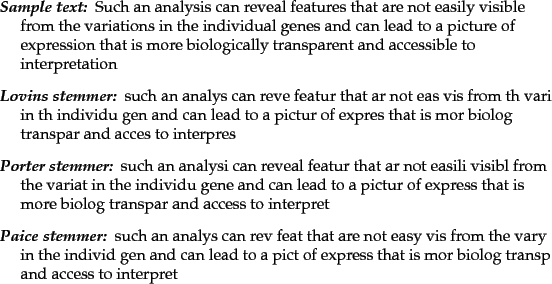
\includegraphics[width=\textwidth]{stemming_examples}
    \end{frame}

    \begin{frame}{Stemming}
        \begin{itemize}
            \item Overstemming - nonsensical stems/different words with the same stems (ex.: university, universal, universities, and universe.)
            \item Understemming - several words that actually are forms of one another (ex.: data, datum -> dat, datu)
        \end{itemize}
    \end{frame}

    \begin{frame}{Stemming for Russian}
        \begin{itemize}
            \item Porter stemmer
            \item Stemka
        \end{itemize}
    \end{frame}

    \begin{frame}{Lemmatization}
       Lemmatization in linguistics is the process of grouping together the inflected forms of a word so they can be analysed as a single item, identified by the word's lemma, or dictionary form.
       \begin{itemize}
           \item uses morhological analysis
           \item resolves a word to its dictionary form (lemma)
           \item saves the part of speech tag (POS-tag) of the word
           \item needs more information, more complex algorithms then for stemming
       \end{itemize}

        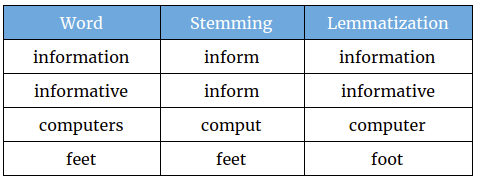
\includegraphics[width=\textwidth]{stemmin_lemm_ex-1.png}
    \end{frame}

       \begin{frame}
  \frametitle{Morphological analysis for Russian}
  \begin{itemize}
  \item Mystem (lemmas, POS-tags, grammatical forms, works with homonyms), R, Python or even with command line
  \item udpipe (+ syntax), R and Python
  \item Stanza (+ syntax), neural algorithm, Python, slower
  \item DeepPavlov (+ syntax), neural algorithm, Python, slower
  \item pymorphy/pymorphy2
  \end{itemize}
\end{frame}




\begin{frame}
  \frametitle{Ambiguity — homonymy of lingistic signs}
  \LARGE
  \begin{block}{Одно слово или разные?}
    Косил \alert<1>{косой косой косой}.
  \end{block}
\only<1>{\normalsize
  коса=S,жен,неод=твор,ед\\
  косая=S,жен,од=(род,ед|дат,ед|твор,ед|пр,ед)\\
  косой=S,муж,од=им,ед\\
  косой=A=(им,ед,полн,муж|род,ед,полн,жен|
  дат,ед,полн,жен|вин,ед,полн,муж,неод|твор,ед,полн,жен| пр,ед,полн,жен)
}
\only<2>{
  \alert{косить}=V,несов=прош,ед,изъяв,муж,пе\\
  \alert{косой}=S,муж,од=им,ед\\
  \alert{косой}=A=твор,ед,полн,жен\\
  \alert{коса}=S,жен,неод=твор,ед
}
\end{frame}

\begin{frame}
    Homonyms are words which are identical in sound form and/or spelling but different in meaning.

    Examples:

    \item Someone left you a \textbf{rose}. - The price \textbf{rose} significantly last month.
    \item You can't \textbf{park} your car here. - Are you heading to the \textbf{park} now?
\end{frame}

    \begin{frame}{Preprocessing steps}
        \begin{enumerate}
            \item Cleaning the data
            \item Tokenization (think about what are the tokens, what to remain and what to drop)
            \item Working with words' forms (stemming/lemmatization/nothing) (what parts of speech to remain?)
            \item Stopwords (to drop or not to drop, how we define stopwords)
        \end{enumerate}

    \end{frame}


    \begin{frame}{Terminology}
          \begin{description}
  \item[corpus] —  collection of texts
  \item[token] — unit of an analysis in the text (for ex.: word)
  \item[wordform] — a word in the text with all its "modifications" - case, tense, etc.
  \item[lexeme] —  a unit of lexical meaning that underlies a set of words that are related through inflection (word in a dictionary, a set of all word forms)
  \item[stemming] — cutting the word to its word stem, base or root form
  \item[lemmatization] — getting the initial form of the word
  \item[POS-tag] - part of speech tag (ex: verb, noun)
  \end{description}
    \end{frame}

       \begin{frame}{Terminology}
          \begin{description}
              \item[corpus size] - the number of all the words/tokens in the corpus (not unique tokens
              \item[vocabulary] - a set of all unique words of the corpus
              \item[vocabulary size] - the number of the unique words/tokens in the corpus
  \end{description}
    \end{frame}


\end{document}

